\documentclass[usenames,dvipsnames,table]{beamer}

\usetheme{CambridgeUS}
\usecolortheme{dolphin}

\usepackage[spanish]{babel}
\usepackage[utf8]{inputenc}
\usepackage[T1]{fontenc}
\usepackage[style=authortitle]{biblatex}
\usepackage{booktabs}
\usepackage{siunitx}
\usepackage{caption}

\usepackage{tikz}
\usetikzlibrary{shapes}
\usetikzlibrary{arrows}

\setbeamertemplate{caption}{\raggedright\insertcaption\par}
\setbeamerfont{caption}{size=\scriptsize}
\setbeamertemplate{navigation symbols}{}

\graphicspath{{../Presentation/figures/}}
\DeclareMathOperator{\ypred}{y_{pred}}
\DeclareMathOperator{\ytrue}{y_{true}}

\DeclareMathOperator{\rank}{rank}
\DeclareMathOperator{\cov}{cov}

\DeclareMathOperator{\TP}{TP}
\DeclareMathOperator{\TN}{TN}
\DeclareMathOperator{\FP}{FP}
\DeclareMathOperator{\FN}{FN}
\DeclareMathOperator{\FPR}{FPR}
\DeclareMathOperator{\AUC}{AUC}
\DeclareMathOperator{\TNR}{TNR}
\DeclareMathOperator{\TNA}{TNA}
\DeclareMathOperator{\TPA}{TPA}
\DeclareMathOperator{\TPR}{TPR}

\DeclareMathOperator{\Precision}{Precision}
\DeclareMathOperator{\Recall}{Recall}
\DeclareMathOperator{\InvPrecision}{Inverse\ Precision}
\DeclareMathOperator{\InvRecall}{Inverse\ Recall}
\DeclareMathOperator{\Accuracy}{Accuracy}

\DeclareMathOperator{\calls}{calls}
\DeclareMathOperator{\etime}{time}
\DeclareMathOperator{\sms}{sms}
\DeclareMathOperator{\contacts}{contacts}

\DeclareMathOperator{\ein}{in}
\DeclareMathOperator{\out}{out}

\DeclareMathOperator{\low}{low}
\DeclareMathOperator{\high}{high}

\DeclareMathOperator{\train}{train}
\DeclareMathOperator{\test}{test}

\DeclareMathOperator{\Betainc}{\Beta_{\operatorname{inc}}}

\DeclareMathOperator{\incalls}{incalls}
\DeclareMathOperator{\outcalls}{outcalls}
\DeclareMathOperator{\insms}{insms}
\DeclareMathOperator{\outsms}{insms}
\DeclareMathOperator{\intime}{outtime}
\DeclareMathOperator{\outtime}{outtime}
\DeclareMathOperator{\incontacts}{incontacts}
\DeclareMathOperator{\outcontacts}{outcontacts}

\DeclareMathOperator{\incallslow}{incallslow}
\DeclareMathOperator{\outcallslow}{outcallslow}
\DeclareMathOperator{\insmslow}{insmslow}
\DeclareMathOperator{\outsmslow}{insmslow}
\DeclareMathOperator{\intimelow}{outtimelow}
\DeclareMathOperator{\outtimelow}{outtimelow}
\DeclareMathOperator{\incontactslow}{incontactslow}
\DeclareMathOperator{\outcontactslow}{outcontactslow}

\DeclareMathOperator{\incallshigh}{incallshigh}
\DeclareMathOperator{\outcallshigh}{outcallshigh}
\DeclareMathOperator{\insmshigh}{insmshigh}
\DeclareMathOperator{\outsmshigh}{insmshigh}
\DeclareMathOperator{\intimehigh}{outtimehigh}
\DeclareMathOperator{\outtimehigh}{outtimehigh}
\DeclareMathOperator{\incontactshigh}{incontactshigh}
\DeclareMathOperator{\outcontactshigh}{outcontactshigh}

\DeclareMathOperator{\neigh}{Neigh}

\DeclareMathOperator{\dir}{dir}
\DeclareMathOperator{\cat}{cat}

\DeclareMathOperator{\ego}{ego}

\DeclareMathOperator{\logit}{logit}

\DeclareMathOperator{\Betadist}{Beta}
\DeclareMathOperator{\Binomial}{Bin}

\addbibresource{../Presentation/sna.bib}

\newcommand{\ct}[1]{\multicolumn{1}{c}{#1}}
\newcommand{\NA}{---}

\title[Algoritmo Copado]{Algoritmo Bayesiano Copado \\ para Encontrar Datos en un Grafo}

\author{Martín~Fixman}
\date{14 Noviembre 2018}

\institute[FCEN UBA]{Facultad de Ciencias Exactas y Naturales \\ Universidad de Buenos Aires}

\begin{document}

\begin{frame}
	\titlepage{}
\end{frame}

\section{El Problema}

\begin{frame}{Fuente de Datos}
	Esta tesis usa dos fuentes de datos principales para cierta población.
	\begin{enumerate}
		\item Dos conjuntos $P$ y $S$ con \emph{Call Detail Records} de llamadas y SMS\@.
		\item Un conjunto $B$ de datos bancarios, del cual se puede extraer el salario mensual.
	\end{enumerate}
\end{frame}

\begin{frame}{Fuente de Datos}
	Con estos datos se calcula el \emph{Grafo Social}.
	\begin{equation*}
		G = \left< \text{V}, \text{E} \right>
	\end{equation*}
	Donde $V$ contiene datos de usuarios y su nivel de ingreso (si se conoce), y $E$ contiene sus conexiones con otros usuarios. Se puede usar el grafo social para entender el comportamiento de los usuarios \footcite{gonzalez2008understanding}\footcite{ponieman2013human}\footcite{sarraute2015city}.

	\begin{center}
		\tikzstyle{white} = [circle, draw, fill=white!25, minimum size=10pt]
\tikzstyle{black} = [circle, draw, fill=black!25, minimum size=10pt]
\tikzstyle{edge} = [draw, thick, >=latex]

\begin{tikzpicture}
	\node[white] (0) at (-2, 0) {};
	\node[black] (1) at (0, 0) {};
	\node[black] (2) at (0, -2) {};
	\node[black] (3) at (-2, -2) {};
	\node[white] (4) at (-1, -1) {};
	\node[black] (5) at (-3, -1) {};
	\path[edge, ->] (0) -- (1);
	\path[edge, ->] (1) -- (2);
	\path[edge, ->] (2) -- (3);
	\path[edge, <->] (3) -- (0);
	\path[edge, ->] (0) -- (4);
	\path[edge, <->] (4) -- (2);
	\path[edge, ->] (4) -- (3);
	\path[edge, <->] (5) -- (0);
	\path[edge, ->] (5) -- (3);

	\node[black] (a) at (1, 0) {};
	\node[white] (e) at (1, -1.5) {};
	\path[edge, <->] (1) -- (a);
	\path[edge, <-] (1) -- (e);
	\path[edge, ->] (2) edge [bend right = 30] (e);

	\path[edge, ->] (e) -- (a);
\end{tikzpicture}

	\end{center}
\end{frame}

\section{Homofilia de Ingresos}

\begin{frame}{Coeficiente de Spearman}
	El Coeficiente de Spearman $r_s$ mide la correlación entre la distribución de dos monotónicas variables $x$ e $y$~\footcite{statistical_analysis}, donde $\rho_{x, y}$ es el \emph{Coeficiente de Pearson} entre $x$ e $y$.


	\begin{equation*}
		r_s = \rho_{\rank\left(x\right), \rank\left(y\right)} = \frac{\cov\left(\rank\left(x\right), \rank\left(y\right)\right)}{\sigma_{\rank(x)} \sigma_{\rank(y)}}
	\end{equation*}

	\onslide<2>{%
		En la fuente de datos usada para esta tesis,

		\begin{equation*}
			r_s = 0.474
		\end{equation*}
	}
\end{frame}

\begin{frame}{Homofilia de Ingresos}
	\begin{figure}
		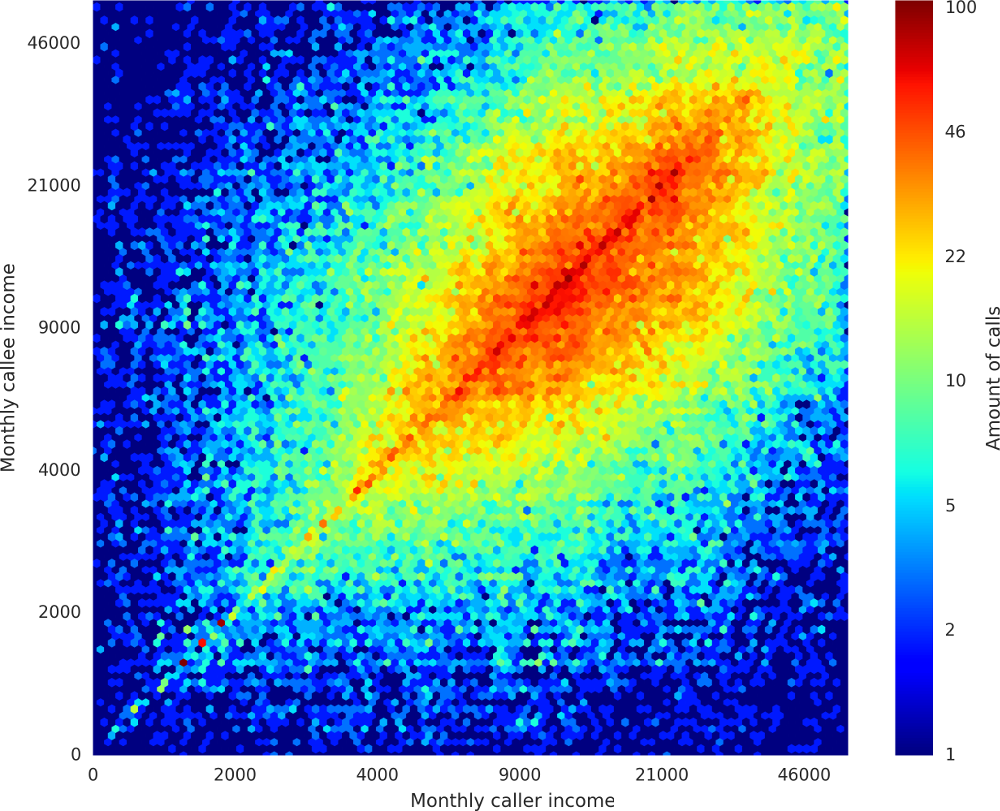
\includegraphics[width=.8\framewidth,height=.75\textheight,keepaspectratio]{heatmap.png}
		\caption{Mapa de calor entre ingresos de usuarios de cada llamada.}
	\end{figure}
\end{frame}

\section{El Modelo Bayesiano}

\begin{frame}{El Modelo Bayesiano}
	\begin{align*}
		H_1 &= \left\{ v \mid v \in V \wedge v_s \leq 6300 \right\} &\text{Usuarios de \emph{Bajos Ingresos}} \\
		H_2 &= \left\{ v \mid v \in V \wedge v_s >    6300 \right\} &\text{Usuarios de \emph{Altos Ingresos}}
	\end{align*}
\end{frame}

\begin{frame}{El Modelo Bayesiano}
	\begin{align*}
		\contacts^{\low}_v &= &\left| \left\{ e \in E \mid e_o = v \land e_d \in H_1 \right\} \cup \left\{ e \in E \mid e_d = v \land e_o \in H_1 \right\} \right| \\
		\contacts^{\high}_v &= &\left| \left\{ e \in E \mid e_o = v \land e_d \in H_2 \right\} \cup \left\{ e \in E \mid e_d = v \land e_o \in H_2 \right\} \right|
	\end{align*}
\end{frame}

\begin{frame}{El Modelo Bayesiano}
	\begin{equation*}
		\varpi \in \left\{ \calls, \etime, \sms, \contacts \right\}
	\end{equation*}
	\pause{}

	En el paper, se demuestra que el reultado óptimo se encuentra cuando $\varpi = \contacts$.
\end{frame}

\begin{frame}{El Modelo Bayesiano}
	Se define una distribución Beta diferente para cada usuario $v \in V$.

	\begin{gather*}
		\Betasim_v \sim B \left( \alt<1-2>{\varpi}{}\alt<3->{\contacts}{}^{\high}_v + 1, \alt<1-2>{\varpi}{}\alt<3->{\contacts}{}^{\low} + 1 \right) \\
		\onslide<2-> {%
		P \left( \Betasim_v \leq x \right) = \frac{1}{B \left( \alt<2>{\varpi}{}\alt<3->{\contacts}{}^{\high} + 1, \alt<2>{\varpi}{}\alt<3->{\contacts}{}^{\low} + 1 \right)} \cdot \int^x_0 {t^{\alt<2>{\varpi}{}\alt<3->{\contacts}{}^{\high}_v} {\left( 1 - t \right)}^{\alt<2>{\varpi}{}\alt<3->{\contacts}{}^{\low}_v} dt}
		}
	\end{gather*}
	\alt<3>{%
		\begin{equation*}
			\bigg( \varpi = \contacts \bigg)
		\end{equation*}
	}{}
	\alt<4->{%
		Para medir la \emph{Incertidumbre}, se elige un cuántil arbitrario $\Theta \in \left[ 0, 1 \right]$ y se define
		\begin{align*}
			p_v &= Q \left( \Theta \right) \\
			&= \inf \left\{ x \in \left[ 0, 1 \right] \mid \Theta \leq F \left( x \right) \right\}
		\end{align*}

		Esta representa la \emph{posterior probability} de $p_v$ dados los datos.
	}{}
\end{frame}

\begin{frame}{El Modelo Bayesiano}
	\begin{figure}
		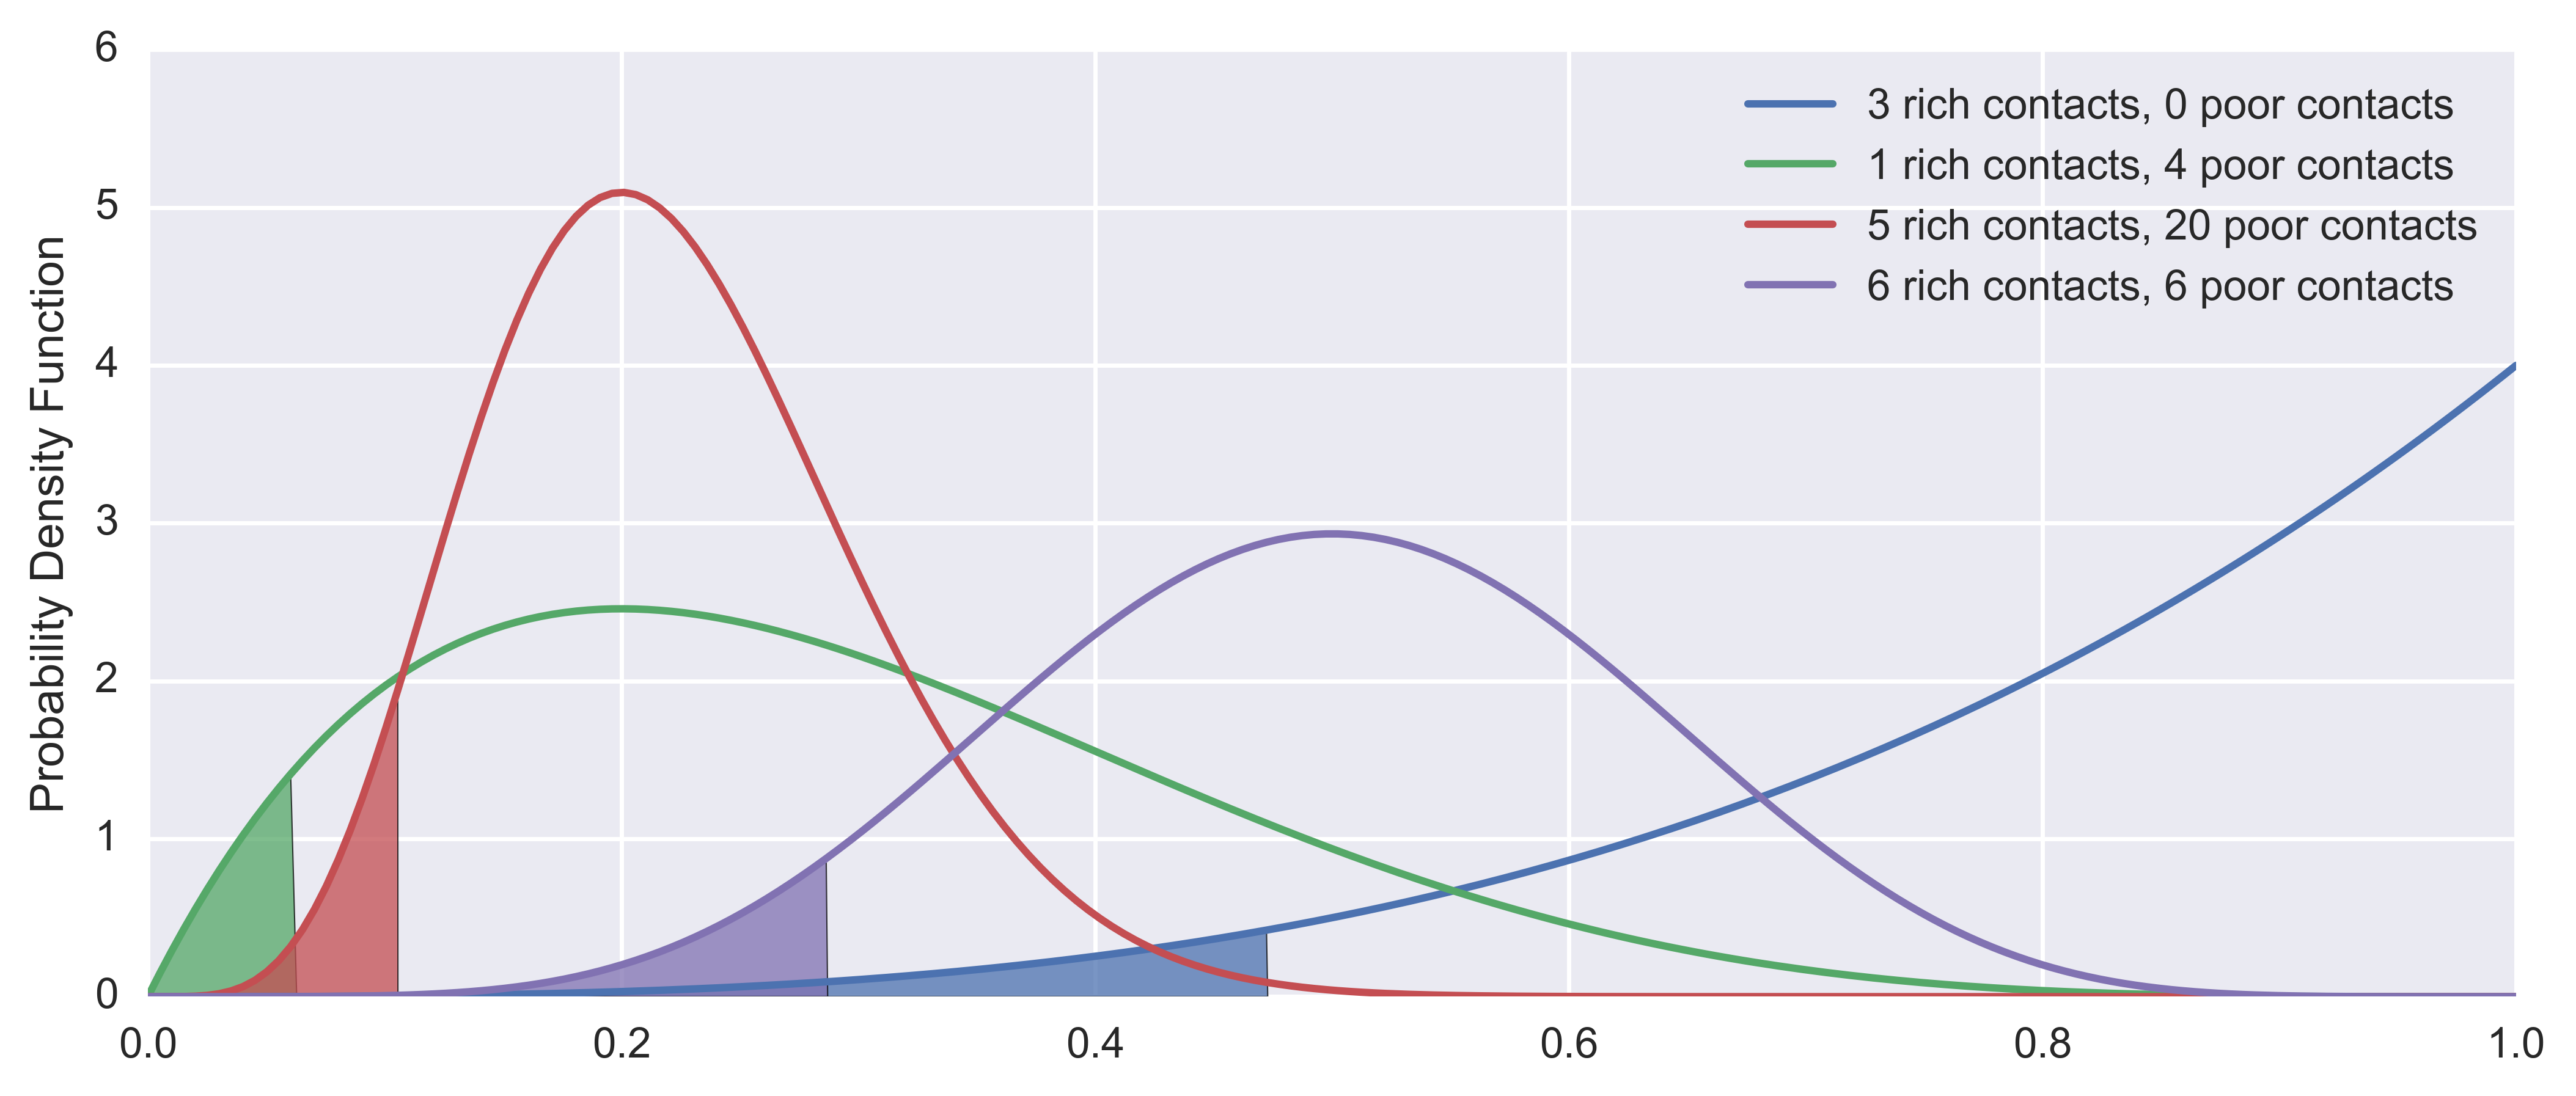
\includegraphics[width=\framewidth,height=0.75\textheight,keepaspectratio]{Beta_example.png}
		\caption{Distribuciones Beta para diferentes usuarios. El área sombreada siempre es igual a $\Theta$, y se integra desde $0$ hasta $p_v$.}
	\end{figure}
\end{frame}

\begin{frame}{El Modelo Bayesiano}
	\onslide<1->{%
		\begin{equation*}
			p_v = Q \left( \Theta \right)
		\end{equation*}
	}
	\onslide<1>{%
		Dados dos usuarios $v$ y $u$, $p_v > p_u$ implica que $v$ tiene mayor probabilidad de tener altos ingresos que $u$.

		Si $u$ tiene altos ingresos y $p_v > p_u$, $v$ tiene altos ingresos.
	}
	\onslide<2->{%
		\begin{gather*}
			\tau \in \left[ 0, 1 \right]  \\
			\vspace{1em} \\
			\begin{aligned}
				p_v \leq \tau &\implies v \in H_1 \\
				p_v >    \tau &\implies v \in H_2
			\end{aligned}
		\end{gather*}

		$\tau$ representa el umbral (threshold) que el algoritmo usa para separar usuarios de bajos y altos ingresos. Este valor puede usarse para incrementar o decrementar la precisión del modelo a cambio de recall.
	}
\end{frame}

\section{Evaluación}

\subsection{Optimizando $\Theta$}

\begin{frame}{Optimizando $\Theta$}
	Para medir la \emph{Incertidumbre}, se elige un cuántil arbitrario $\Theta \in \left[ 0, 1 \right]$ y se define
	\begin{align*}
		p_v &= Q \left( \Theta \right) \\
		&= \inf \left\{ x \in \left[ 0, 1 \right] \mid \Theta \leq F \left( x \right) \right\}
	\end{align*}

	Esta representa la \emph{posterior probability} de $p_v$ dados los datos.

	\pause{}
	Cuando $\varpi = \contacts$,
	\begin{table}
		\begin{tabular}{l r r}
			\toprule
			\ct{$\varpi$}& \ct{$\Theta$ Óptimo} & \ct{AUC} \\
			\midrule
			contacts & \num{0.394} & \num{0.746} \\
			\bottomrule
		\end{tabular}
		\caption{Resultados para $\Theta$ que maximizan el \emph{área bajo la curva}.}
	\end{table}
\end{frame}

\subsection{Optimizando $\tau$}

\begin{frame}{Optimizando $\tau$}
	\begin{itemize}
		\item Eligiendo un $\varpi$ y dado un $\Theta$, ya tenemos un buen modelo de predicción para $p_v$, la probabilidad de que $v$ sea un usuario de altos ingresos.
		\item $\tau$ representa el umbral (threshold) que el algoritmo usa para separar usuarios de bajos y altos ingresos.
			\begin{gather*}
				\begin{aligned}
					p_v \leq \tau &\implies v \in H_1 \\
					p_v >    \tau &\implies v \in H_2
				\end{aligned}
			\end{gather*}
		\item Para cada $\varpi$, se elige el $\tau$ que maximice la \emph{exactitud} (accuracy) del modelo.
	\end{itemize}
\end{frame}

\subsection{Optimizando $\varpi$}

\begin{frame}{Infiriendo por Cantidad de Contactos}

	\begin{figure}
		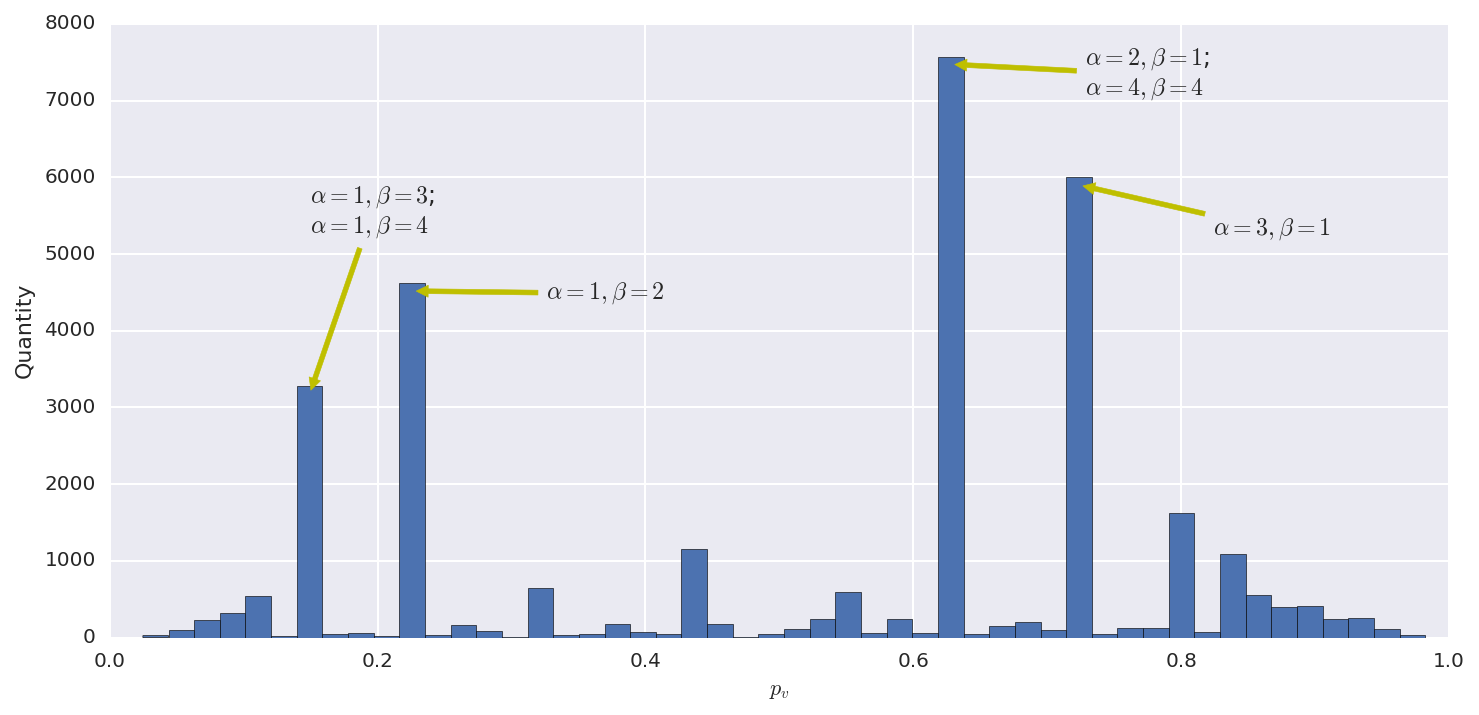
\includegraphics[width=\framewidth, height=.37\textheight, keepaspectratio]{bayes/hist_contacts.png} \\
		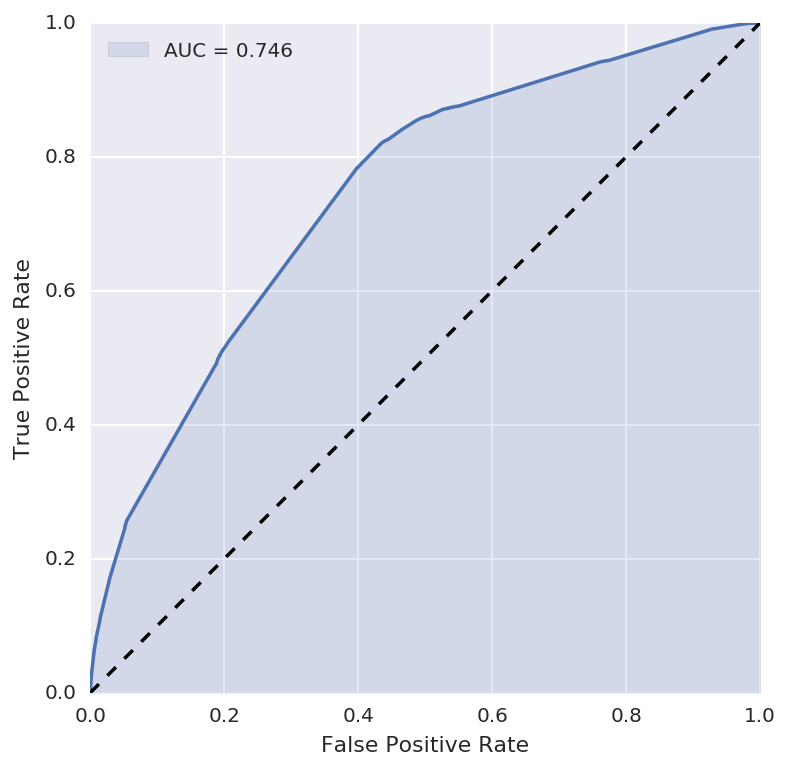
\includegraphics[width=.49\framewidth, height=.37\textheight, keepaspectratio]{bayes/roc_contacts.png}
		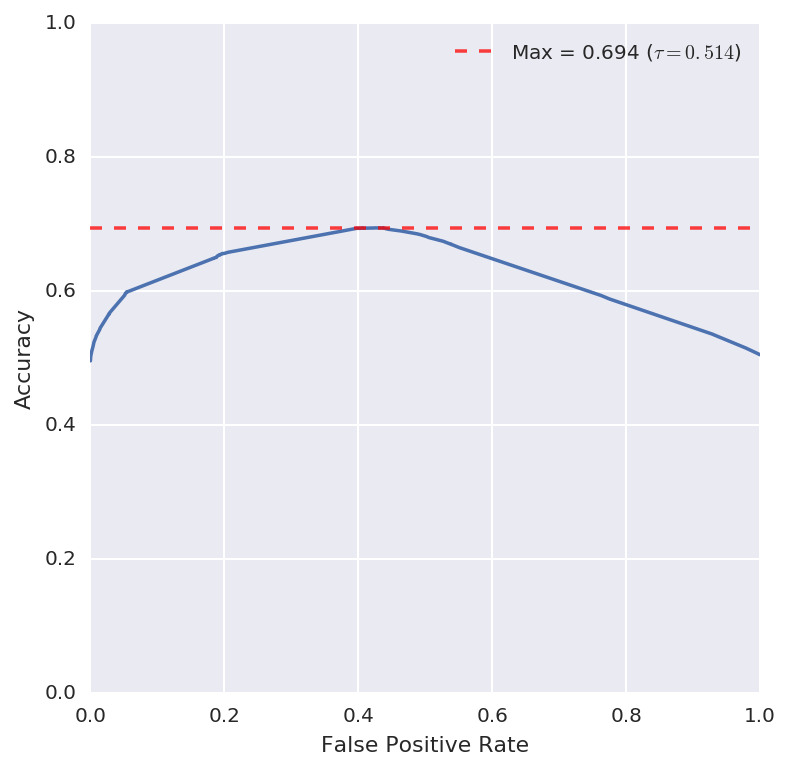
\includegraphics[width=.49\framewidth, height=.37\textheight, keepaspectratio]{bayes/accuracy_contacts.png}

		\caption{Resultados del \emph{método bayesiano} usando el grado de cada usuario. $\tau = 0.514$}
	\end{figure}

\end{frame}

\subsection{Resultados Finales}

\begin{frame}{Resultados Finales}
	\begin{table}
		\begin{tabular}{l r r r r r r r r}
			\toprule
			$\varpi$ & \ct{$\Theta$} & \ct{$\tau$} & \ct{Acc.} & \ct{Prec.} & \ct{Rec.} & \ct{AUC} & \ct{F\textsubscript{1}} & \ct{F\textsubscript{4}} \\
			\midrule
			calls    & 0.428 & 0.654 & 0.686 & 0.654 & 0.816 & 0.724 & 0.726 & 0.804 \\
			time     & 0.001 & 0.722 & 0.681 & 0.652 & 0.806 & 0.718 & 0.721 & 0.795 \\
			sms      & 0.428 & 0.299 & 0.688 & 0.648 & 0.789 & 0.715 & 0.712 & 0.779 \\
			contacts & 0.394 & 0.514 & 0.693 & 0.665 & 0.792 & 0.746 & 0.723 & 0.783 \\
			\bottomrule
		\end{tabular}
		\caption{Metrics for the Bayesian algorithm using every user in $\Upsilon$}
	\end{table}

	\pause{}
	Las mejores métricas del algoritmo se van para estos hiperparámetros.
	\begin{align*}
		\varpi &= \contacts \\
		\Theta &= 0.394 \\
		\tau &= 0.514
	\end{align*}
\end{frame}


\end{document}
